% Provenance (never printed): old premiere S material on the lithosphere and the
% asthenosphere (chemical and mechanical layers, the low-velocity zone, the
% geotherm, isostasy); see sources/book2/PROVENANCE.md. S speeds from
% figdata/grade-11/prem_profiles.py (part upper), the geotherm and the solidus
% from geotherm_solidus.py, the elevations from hypsometry.py (ETOPO1).
% Glacial rebound belongs to g12; lithostatic pressure (term) to g12.
\chapter{Litosfera y astenosfera}\label{ch:g11:lithosphere-asthenosphere}

Nueve décimas partes de un iceberg están bajo el agua: el hielo flota porque
es un poco menos denso que el mar, y se hunde en el agua hasta que el agua
que aparta pesa tanto como todo el iceberg. Las cordilleras se comportan más o
menos igual. Bajo las más altas, la corteza tiene casi el doble del espesor
habitual, y la mayor parte de esa corteza de más queda oculta debajo, como el hielo bajo
la línea de flotación. Pero un iceberg flota en un líquido, y el manto que hay
bajo una cordillera es roca sólida. Este capítulo muestra cómo un sólido puede
comportarse como un fluido sobre el que flota la capa externa de la Tierra, y
qué es esa capa.
% ledger: usgs:ice-density, karplus:tibet-moho, cm95:crust

\begin{recall}
La Tierra tiene una corteza, un manto y un núcleo (Libro 1, año 6). El \omterm{def:g11:seismic-structure:moho}{Moho},
en la base de la corteza, está de media a unos \qty{41}{km} de profundidad
bajo los continentes y a pocos kilómetros bajo el fondo oceánico; las
velocidades sísmicas y las densidades se conocen a cada profundidad gracias a
un \omterm{def:g11:seismic-structure:reference-model}{modelo terrestre de referencia} (el \cref{ch:g11:seismic-structure}). La
roca se calienta con la profundidad, unos 25 a \qty{30}{\celsius} por
kilómetro cerca de la superficie (Libro 1, año 6). Un cuerpo que flota en un
líquido aparta un peso de líquido igual a su propio peso, y la presión en el
fondo de una columna de material es el peso de la columna dividido entre su
área (los libros de física).
\end{recall}
% ledger: cm95:crust, usgs:crust-thickness, usgs:gradient-29 (Book 1 rows)

\begin{omfigure}
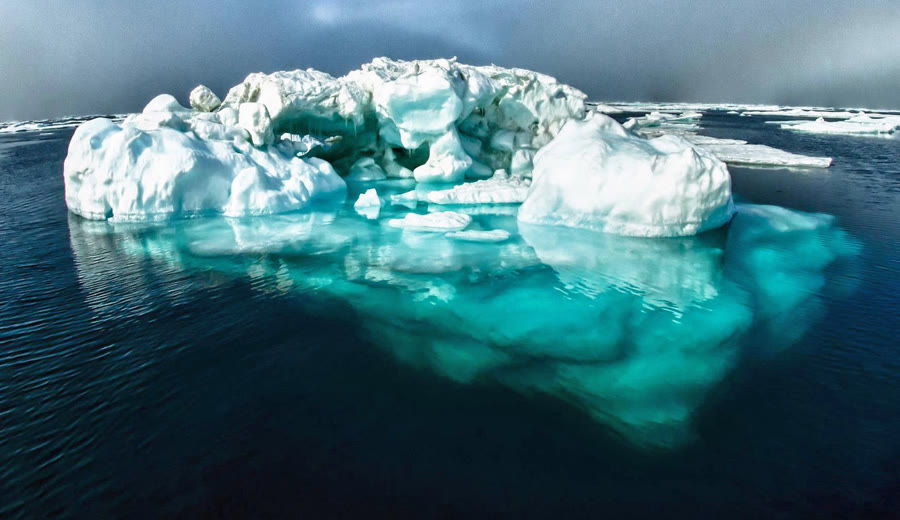
\includegraphics[width=0.66\linewidth]{images/book2/g11-noaa-iceberg.jpg}

{\small Un iceberg visto justo por encima del agua: el hielo sumergido, que se
transparenta en el mar claro, es mucho mayor que la parte que asoma al aire.
Fotografía: NOAA (dominio público).}
\end{omfigure}
% ledger: photo:g11-iceberg

\section{Dos maneras de dividir la Tierra en capas}

La corteza, el manto y el núcleo son capas de \emph{materiales} distintos: la
corteza está hecha de rocas ricas en silicio, aluminio y oxígeno; el manto, de
una roca más densa; el núcleo, de metal. Pero la parte externa de la Tierra
también puede dividirse según cómo se \emph{comporta} su roca cuando actúan
sobre ella fuerzas durante muchísimo tiempo.

\begin{definition}[Litosfera; astenosfera]\label{def:g11:lithosphere-asthenosphere:lithosphere}
La \emph{litosfera}\index{litosfera} es la capa externa rígida de la Tierra:
la corteza y la parte más alta y más fría del manto, que juntas se rompen en
las placas tectónicas y no fluyen. La
\emph{astenosfera}\index{astenosfera} es la capa del manto situada bajo la
litosfera, más caliente y más débil, que fluye
lentamente a lo largo de mucho tiempo, como una pasta muy espesa.
\end{definition}

El límite entre las dos está a unos 70 a \qty{100}{km} de profundidad bajo los
océanos y la mayoría de los continentes, y más hondo bajo las partes más
antiguas de los continentes; a lo ancho de Estados Unidos, por ejemplo, la
\omterm{def:g11:lithosphere-asthenosphere:lithosphere}{litosfera} pasa de unos \qty{40}{km} de espesor en el oeste a más de
\qty{200}{km} en el centro del continente. La base de la \omterm{def:g11:lithosphere-asthenosphere:lithosphere}{litosfera} no es el
\omterm{def:g11:seismic-structure:moho}{Moho}: la mayor parte de la \omterm{def:g11:lithosphere-asthenosphere:lithosphere}{litosfera} es roca del manto.
% ledger: rs09:lab, fischer:lab, porter:lab, usgs:lithosphere-80km (Book 1 row)

\begin{omfigure}
\begin{tikzpicture}[x=1cm, y=-0.0125cm, font=\footnotesize]
% depths to scale: crust 41 km (cm95:crust), lithosphere 100 km (rs09:lab), 0-400 km
  \shade[top color=omLithPeridotite!70, bottom color=omLithPeridotite!25] (5,100) rectangle (8,400);
  \fill[omLithGranite!55] (0,0) rectangle (3,41);
  \fill[omLithPeridotite!55] (0,41) rectangle (3,400);
  \fill[black!25] (5,0) rectangle (8,100);
  \draw (0,0) rectangle (3,400);
  \draw (5,0) -- (5,400) (8,0) -- (8,400) (5,0) -- (8,0);
  \draw[line width=0.8pt] (0,41) -- (3,41);
  \draw[line width=0.8pt, densely dashed] (5,100) -- (8,100);
  \draw[densely dotted, black!60] (3,41) -- (5,41);
  \node at (1.5,20) {corteza};
  \node[align=center] at (1.5,220) {manto};
  \node[align=center] at (6.5,50) {litosfera\\rígida};
  \node[align=center] at (6.5,180) {astenosfera\\débil, fluye despacio};
  \node[align=center, text=black!70] at (6.5,340) {manto más profundo};
  \node[anchor=south, font=\small] at (1.5,0) {por material};
  \node[anchor=south, font=\small] at (6.5,0) {por comportamiento};
  \foreach \d in {0,100,200,300,400} {\draw (-0.1,\d) -- (0,\d); \node[anchor=east] at (-0.1,\d) {\d};}
  \node[anchor=east, rotate=90, anchor=south] at (-0.9,200) {profundidad (\unit{km})};
  \node[anchor=south, font=\scriptsize, align=center] at (4,41) {Moho\\(\qty{41}{km})};
  \node[anchor=west, align=left] at (8.15,100) {base de la\\litosfera\\(unos \qty{100}{km})};
\end{tikzpicture}

{\small Los \qty{400}{km} superiores de la Tierra bajo un continente, a escala.
A la izquierda: las capas según el material. A la derecha: las capas según el
comportamiento. La \omterm{def:g11:lithosphere-asthenosphere:lithosphere}{litosfera} rígida contiene toda la corteza y la parte alta
del manto; la \omterm{def:g11:lithosphere-asthenosphere:lithosphere}{astenosfera} no tiene un límite inferior neto.}
\end{omfigure}

\section{La zona de baja velocidad}

Las ondas sísmicas muestran la \omterm{def:g11:lithosphere-asthenosphere:lithosphere}{astenosfera}. En casi todo el interior de la
Tierra, las velocidades sísmicas aumentan con la profundidad, porque la roca
está cada vez más comprimida. Bajo la \omterm{def:g11:lithosphere-asthenosphere:lithosphere}{litosfera} ocurre lo contrario.

\begin{definition}[Zona de baja velocidad]\label{def:g11:lithosphere-asthenosphere:lvz}
La \emph{zona de baja velocidad}\index{zona de baja velocidad} es la capa del
manto superior, bajo la \omterm{def:g11:lithosphere-asthenosphere:lithosphere}{litosfera}, en la que las ondas sísmicas viajan más
despacio que en la roca de encima y de debajo.
\end{definition}

En el \omterm{def:g11:seismic-structure:reference-model}{modelo terrestre de referencia}, la velocidad S baja lentamente desde el
\omterm{def:g11:seismic-structure:moho}{Moho} hasta \qty{220}{km}, y luego salta hacia arriba. Los estudios sísmicos
de todo el mundo encuentran una caída brusca de la velocidad en algún punto
entre 70 y \qty{100}{km}: el techo de la \omterm{def:g11:lithosphere-asthenosphere:lithosphere}{astenosfera}. La roca está allí lo
bastante caliente como para estar cerca de fundirse, y puede contener una
cantidad ínfima de fundido; también puede contener más agua que la roca de
encima. Una roca cercana a la fusión es débil: frena las ondas sísmicas y
puede fluir.
% ledger: data:prem, rs09:lab, fischer:lab, porter:lab

\begin{omfigure}
\begin{tikzpicture}
\begin{axis}[omrecord, omdepth, width=0.6\linewidth, height=6.0cm, xmin=3.0, xmax=5.0, ymin=0, ymax=400,
  xlabel={velocidad S (\unit{km/s})}, ylabel={profundidad (\unit{km})}, xtick={3.0,3.5,...,5.0},
  xticklabel style={/pgf/number format/fixed, /pgf/number format/precision=1},
  tick label style={font=\small}, label style={font=\small}]
% computed in figdata/grade-11/prem_profiles.py (part upper); ledger: data:prem
\fill[black!10] (axis cs:3.0,80) rectangle (axis cs:5.0,220);
\addplot[omProp, line width=0.9pt] table[x=vs, y=depth] {figdata/out/grade-11-prem_profiles-upper.dat};
\node[font=\scriptsize, anchor=west, align=left] at (axis cs:3.1,150) {zona de\\baja velocidad};
\node[font=\scriptsize, anchor=west] at (axis cs:3.95,12) {corteza};
\end{axis}
\end{tikzpicture}

{\small La velocidad S en los \qty{400}{km} superiores del \omterm{def:g11:seismic-structure:reference-model}{modelo terrestre de
referencia}. Bajo la corteza, la velocidad disminuye lentamente con la
profundidad hasta \qty{220}{km} (sombreado a partir de \qty{80}{km}), y luego
vuelve a aumentar con saltos bruscos.}
\end{omfigure}

\section{La geoterma}

\begin{definition}[Geoterma; gradiente geotérmico]\label{def:g11:lithosphere-asthenosphere:geotherm}
Una \emph{geoterma}\index{geoterma} es la curva de la temperatura en función
de la profundidad bajo un lugar. El \emph{gradiente
geotérmico}\index{gradiente geotermico@gradiente geotérmico} es el aumento de
la temperatura por unidad de profundidad, en grados por kilómetro.
\end{definition}

Los sondeos solo miden la \omterm{def:g11:lithosphere-asthenosphere:geotherm}{geoterma} en los primeros kilómetros, donde la
temperatura sube de 25 a \qty{30}{\celsius} por kilómetro (Libro 1,
año 6). Más abajo se calcula a partir del calor que sale por la superficie y
de las propiedades de las rocas; el \cref{ch:g12:internal-heat}
muestra de dónde viene ese calor. Dos hechos determinan el resultado. Parte
del calor se produce dentro de la propia corteza superior, así que el
gradiente es más fuerte cerca de la superficie y menor bajo la corteza. Y en
la \omterm{def:g11:lithosphere-asthenosphere:lithosphere}{astenosfera}, que fluye, el lento movimiento de la roca transporta el calor
e iguala la temperatura: solo sube unos \qty{0.45}{\celsius} por kilómetro. La
base de la \omterm{def:g11:lithosphere-asthenosphere:lithosphere}{litosfera} se sitúa donde la \omterm{def:g11:lithosphere-asthenosphere:geotherm}{geoterma} empinada de la \omterm{def:g11:lithosphere-asthenosphere:lithosphere}{litosfera} se
encuentra con la \omterm{def:g11:lithosphere-asthenosphere:geotherm}{geoterma} suave de la \omterm{def:g11:lithosphere-asthenosphere:lithosphere}{astenosfera}, hacia los
\qty{1300}{\celsius}.
% ledger: usgs:gradient-29 (Book 1 row), b2dd10:continents, b2roy:provinces, roy:conductivity,
% katsura10:adiabat, porter:lab

\begin{omfigure}
\begin{tikzpicture}
\begin{axis}[omrecord, omdepth, width=0.7\linewidth, height=6.4cm, xmin=0, xmax=2000, ymin=0, ymax=300,
  xlabel={temperatura (\unit{\celsius})}, ylabel={profundidad (\unit{km})}, xtick={0,500,...,2000},
  tick label style={font=\small}, label style={font=\small}]
% computed in figdata/grade-11/geotherm_solidus.py; ledger: b2dd10:continents, b2roy:provinces,
% roy:conductivity, porter:lab, katsura10:adiabat, hirschmann:solidus, data:prem
\fill[black!8] (axis cs:0,99.7) rectangle (axis cs:2000,300);
\addplot[omDef, line width=1.0pt] table[x=t_geotherm, y=depth_km] {figdata/out/grade-11-geotherm_solidus-geotherm.dat};
\addplot[omDef, densely dashed, restrict y to domain=99:300] table[x=t_cond, y=depth_km] {figdata/out/grade-11-geotherm_solidus-geotherm.dat};
\addplot[omProp, line width=1.0pt] table[x=t_solidus, y=depth_km] {figdata/out/grade-11-geotherm_solidus-geotherm.dat};
\draw[black!60] (axis cs:0,99.7) -- (axis cs:2000,99.7);
\node[font=\scriptsize, anchor=south west] at (axis cs:20,99.7) {base de la litosfera};
\node[font=\scriptsize, anchor=north west] at (axis cs:20,102) {astenosfera};
\node[font=\scriptsize, text=omDef, anchor=north west] at (axis cs:480,6) {geoterma};
\node[font=\scriptsize, text=omProp, anchor=west] at (axis cs:1300,22) {empieza la fusión};
\end{axis}
\end{tikzpicture}

{\small Una \omterm{def:g11:lithosphere-asthenosphere:geotherm}{geoterma} modelo bajo un continente (azul) y la temperatura a la
que la roca del manto (peridotita, sin agua) empieza a fundirse (naranja). La
\omterm{def:g11:lithosphere-asthenosphere:geotherm}{geoterma} se calcula a partir del flujo de calor medio de los continentes y de
propiedades medidas de las rocas; en la \omterm{def:g11:lithosphere-asthenosphere:lithosphere}{astenosfera} (gris) sube despacio. La línea discontinua muestra
cómo seguiría la subida más empinada de la \omterm{def:g11:lithosphere-asthenosphere:lithosphere}{litosfera}. Las dos curvas se
acercan más, a unos \qty{140}{\celsius} una de otra, cerca de la base de la
\omterm{def:g11:lithosphere-asthenosphere:lithosphere}{litosfera}.}
\end{omfigure}
% values: lab_km 99.7, t_lab_c 1345, closest_gap_c 144 (figdata/grade-11/geotherm_solidus.py)

La temperatura de fusión de la roca del manto sube con la profundidad, porque
la roca está cada vez más comprimida (Libro 1, año 6): unos
\qty{1120}{\celsius} en la superficie, casi \qty{1500}{\celsius} a
\qty{100}{km}. En el modelo, la \omterm{def:g11:lithosphere-asthenosphere:geotherm}{geoterma} se acerca más a ella justo bajo la
\omterm{def:g11:lithosphere-asthenosphere:lithosphere}{litosfera}, a unos \qty{140}{\celsius} por debajo. Un poco de agua, o un manto
algo más caliente, cierra la diferencia: en el oeste de Estados Unidos, donde
la \omterm{def:g11:lithosphere-asthenosphere:lithosphere}{litosfera} es delgada, una pequeña parte del manto de debajo está
parcialmente fundida.
% ledger: hirschmann:solidus, porter:lab; computed in figdata/grade-11/geotherm_solidus.py
% (solidus0_c 1120.7, solidus100_c 1489, closest_gap_c 144)

\section{La isostasia}

\subsection{Flotar sobre un sólido}

Durante los pocos segundos que dura una onda sísmica, la \omterm{def:g11:lithosphere-asthenosphere:lithosphere}{astenosfera} es un
sólido. A lo largo de mucho tiempo, fluye. Una carga colocada sobre la
\omterm{def:g11:lithosphere-asthenosphere:lithosphere}{litosfera} --- una cordillera, un casquete de hielo --- aparta lentamente la
\omterm{def:g11:lithosphere-asthenosphere:lithosphere}{astenosfera} hasta que la carga flota, como un bloque de madera en el agua.

\begin{definition}[Isostasia; profundidad de compensación]\label{def:g11:lithosphere-asthenosphere:isostasy}
La \emph{isostasia}\index{isostasia} es el equilibrio en el que las capas
externas de la Tierra flotan sobre la \omterm{def:g11:lithosphere-asthenosphere:lithosphere}{astenosfera}: a una profundidad del manto
llamada \emph{profundidad de compensación}\index{profundidad de compensacion@profundidad de compensación},
todas las columnas de roca de la misma sección, desde la superficie hasta esa
profundidad, tienen el mismo peso, sea cual sea el relieve que haya encima.
\end{definition}

\begin{omfigure}
\begin{tikzpicture}[x=1cm, y=1cm, font=\footnotesize, >={Stealth[length=4pt]}]
% not to scale
  \fill[omSea!50] (6,0) rectangle (8.6,-0.9);
  \fill[omLithPeridotite!45] (0,-5.2) rectangle (2.6,-6.6);
  \fill[omLithGranite!55] (0,2.0) -- (2.6,2.0) -- (2.6,-5.2) -- (0,-5.2) -- cycle;
  \fill[omLithGranite!55] (2.6,0) rectangle (6,-3.0);
  \fill[omLithGranite!55] (6,-0.9) rectangle (8.6,-1.6); % same fill: one crustal density in Airy's model
  \fill[omLithPeridotite!45] (2.6,-3.0) rectangle (6,-6.6);
  \fill[omLithPeridotite!45] (6,-1.6) rectangle (8.6,-6.6);
  \draw (0,2.0) -- (2.6,2.0) -- (2.6,0) -- (6,0);
  \draw (6,0) -- (8.6,0);
  \draw[line width=0.8pt] (0,-5.2) -- (2.6,-5.2) -- (2.6,-3.0) -- (6,-3.0) -- (6,-1.6) -- (8.6,-1.6);
  \draw[densely dashed, line width=0.8pt] (0,-6.2) -- (8.6,-6.2);
  \node[anchor=north east] at (8.6,-6.6) {profundidad de compensación};
  \draw[black!50, densely dotted] (-0.2,0) -- (0,0);
  \node[anchor=east] at (-0.2,0) {nivel del mar};
  \node at (1.3,-1.6) {corteza};
  \node at (4.3,-1.5) {corteza};
  \node at (7.3,-0.45) {océano};
  \node at (7.3,-1.25) {corteza};
  \node at (4.3,-4.8) {manto};
  \node[anchor=south] at (1.3,2.0) {cordillera};
  \node[anchor=south] at (4.3,0) {llanura};
  \draw[<->] (2.75,0) -- (2.75,2.0); \node[anchor=west] at (2.8,1.0) {$h$};
  \draw[<->] (2.75,-3.0) -- (2.75,-5.2); \node[anchor=west] at (2.8,-4.1) {raíz $r$};
  \draw[<->] (5.85,0) -- (5.85,-3.0); \node[anchor=east] at (5.8,-1.0) {$T$};
\end{tikzpicture}

{\small El modelo de \omterm{prop:g11:lithosphere-asthenosphere:airy}{isostasia de Airy} (sin escala). La corteza tiene en todas
partes la misma densidad; donde está alta, es gruesa y tiene una raíz que se
hunde profundamente en el manto, más denso. Bajo el océano, la corteza es
delgada. Las tres columnas pesan lo mismo hasta la \omterm{def:g11:lithosphere-asthenosphere:isostasy}{profundidad de
compensación}.}
\end{omfigure}

\subsection{La raíz de una cordillera}

\begin{proposition}[Isostasia de Airy]\label{prop:g11:lithosphere-asthenosphere:airy}
Supongamos que la corteza tiene una densidad uniforme $\rho_c$, y el manto de
debajo una densidad $\rho_m > \rho_c$. Si una región está a una altura $h$ por
encima de otra y las dos están en equilibrio isostático, su corteza es más
gruesa en
\[
  \Delta H = h\,\frac{\rho_m}{\rho_m - \rho_c},
\]
de los que $h$ sobresalen por encima de la otra región y una raíz
$r = h\,\rho_c/(\rho_m - \rho_c)$ se hunde por debajo de su corteza.\index{isostasia de Airy}
\end{proposition}

\begin{proof}
Tomemos dos columnas de la misma área $S$: la llanura, con una corteza de
espesor $T$, y la cordillera, cuya corteza sobresale $h$ más arriba y llega
$r$ más abajo, de modo que su espesor es $T + h + r$. Hasta una \omterm{def:g11:lithosphere-asthenosphere:isostasy}{profundidad de
compensación} situada por debajo de los dos \omterm{def:g11:seismic-structure:moho}{Mohos}, la columna de la cordillera
tiene $h + r$ más de corteza; la columna de la llanura tiene, en cambio, manto
en el espesor $r$. Con $g$ la aceleración de la gravedad, los dos pesos son
iguales cuando
\[
  \rho_c\,(h + r)\,S\,g = \rho_m\,r\,S\,g,
  \qquad\text{es decir}\qquad
  r = h\,\frac{\rho_c}{\rho_m - \rho_c}.
\]
La corteza es más gruesa en $h + r = h\,\bigl(1 + \rho_c/(\rho_m - \rho_c)\bigr)
= h\,\rho_m/(\rho_m - \rho_c)$.
\end{proof}

Con la densidad media de la corteza continental, $\rho_c =
\qty{2830}{kg/m^3}$, y la del manto justo bajo el \omterm{def:g11:seismic-structure:moho}{Moho}, $\rho_m =
\qty{3380}{kg/m^3}$, la raíz es $2830/550 \approx 5.1$ veces la altura, y la
corteza es más gruesa en unas $6.1$ veces la altura: una cordillera que se
eleva \qty{3}{km} sobre sus alrededores tiene una raíz de unos \qty{15}{km}.
% ledger: cm95:crust, data:prem (rho 3.38 below the Moho)

\begin{method}[Calcular una raíz]\label{met:g11:lithosphere-asthenosphere:root}
\begin{enumerate}
  \item Busca la altura $h$ de la región por encima de una región de
        referencia cuyo espesor de corteza se conoce.
  \item Calcula $\rho_m/(\rho_m - \rho_c)$ con las densidades de la corteza y
        del manto.
  \item La corteza es más gruesa que la de referencia en $h\,\rho_m/(\rho_m -
        \rho_c)$; la raíz sola es eso menos $h$.
\end{enumerate}
\end{method}

\begin{example}[Una meseta de \qty{2}{km} de altura]\label{ex:g11:lithosphere-asthenosphere:plateau}
Una meseta se eleva \qty{2}{km} sobre una llanura cuya corteza tiene
\qty{37}{km} de espesor. Su corteza es más gruesa en $2 \times 3380/550 \approx \qty{12.3}{km}$:
unos \qty{49}{km} en total, con una raíz de unos \qty{10}{km}.
\end{example}

\subsection{Por qué los continentes están altos}

\begin{definition}[Curva hipsométrica]\label{def:g11:lithosphere-asthenosphere:hypsometry}
La \emph{curva hipsométrica}\index{curva hipsometrica@curva hipsométrica} de
la Tierra da, para cada altitud, la fracción de la superficie de la Tierra
que está por encima de ella. Su pendiente muestra cuánta superficie hay a cada
altitud.
\end{definition}

Si la superficie se hubiera modelado al azar, casi toda estaría cerca de un
nivel medio. No es así.

\begin{proposition}[Dos niveles]\label{prop:g11:lithosphere-asthenosphere:two-levels}
Las altitudes de la superficie de la Tierra se agrupan en torno a dos niveles:
uno a pocos cientos de metros del nivel del mar, en los continentes, y otro a
unos 4 a \qty{5}{km} por debajo del nivel del mar, en el fondo oceánico
profundo. Las tierras emergidas cubren el \qty{29}{\percent}
de la superficie; más de la mitad de la superficie está a más de \qty{3}{km}
por debajo del nivel del mar, y solo el \qty{3}{\percent} se eleva a más de
\qty{2}{km}.
\end{proposition}
% computed in figdata/grade-11/hypsometry.py from ETOPO1 (land_fraction 0.290,
% share_below_3000_pct 53.4, share_above_2000_pct 3.1; modes at +250 and -4250 m); ledger: data:etopo1

\begin{omfigure}
\begin{tikzpicture}
\begin{axis}[omrecord, width=0.86\linewidth, height=5.4cm, xmin=-11000, xmax=9000, ymin=0, ymax=18,
  xlabel={altitud (\unit{m}; negativa: bajo el nivel del mar)}, ylabel={parte de la superficie (\unit{\percent})},
  xtick={-10000,-8000,...,8000}, scaled x ticks=false, xticklabel style={/pgf/number format/1000 sep={\,}, font=\scriptsize},
  tick label style={font=\small}, label style={font=\small}, clip=false]
% computed in figdata/grade-11/hypsometry.py; ledger: data:etopo1
\addplot[ybar interval, fill=omSea!70, draw=black!50, restrict expr to domain={\thisrow{land}}{0:0}] table[x=lo, y=share_pct] {figdata/out/grade-11-hypsometry-bins.dat};
\addplot[ybar interval, fill=omHypsLandC, draw=black!50, restrict expr to domain={\thisrow{land}}{1:1}] table[x=lo, y=share_pct] {figdata/out/grade-11-hypsometry-bins.dat};
\draw[black!60, densely dotted] (axis cs:0,0) -- (axis cs:0,18);
\node[font=\scriptsize, anchor=south west] at (axis cs:600,15.5) {continentes};
\node[font=\scriptsize, anchor=south] at (axis cs:-4250,12.2) {fondo oceánico profundo};
\end{axis}
\end{tikzpicture}

{\small Parte de la superficie de la Tierra en cada franja de \qty{500}{m} de
altitud (según ETOPO1, a un grado; sobre la Antártida y Groenlandia, la parte
alta del hielo). Los dos picos son los continentes y el fondo oceánico
profundo.}
\end{omfigure}

La \omterm{def:g11:lithosphere-asthenosphere:isostasy}{isostasia} explica los dos niveles. Los continentes están hechos de una
corteza gruesa, de unos \qty{41}{km} de media, de roca ligera; el fondo
oceánico, de una corteza delgada de roca más densa, de solo unos \qty{5}{km}
de espesor. Las dos flotan sobre la \omterm{def:g11:lithosphere-asthenosphere:lithosphere}{astenosfera}: la corteza continental,
gruesa y ligera, flota alta; la corteza oceánica, delgada y densa, flota baja,
y los océanos llenan las tierras bajas.
% ledger: cm95:crust, usgs:crust-thickness (Book 1 row)

\section{Una tapa flexible}

La \omterm{def:g11:lithosphere-asthenosphere:isostasy}{isostasia} necesita que la \omterm{def:g11:lithosphere-asthenosphere:lithosphere}{astenosfera} fluya. La \omterm{def:g11:lithosphere-asthenosphere:lithosphere}{litosfera} de encima no
fluye: se dobla. Una carga más estrecha que el espesor de la \omterm{def:g11:lithosphere-asthenosphere:lithosphere}{litosfera}, como
una sola isla volcánica, la sostiene la rigidez de la placa, como un peso
sobre un tablón, y la placa se hunde a su alrededor. Una carga mucho más
ancha que ese espesor, como toda una cordillera o un casquete de hielo, se
hunde hasta flotar. Cuando se retira la carga, la \omterm{def:g11:lithosphere-asthenosphere:lithosphere}{litosfera} vuelve a subir
lentamente (el \cref{ch:g12:destruction-of-mountains}).

\section{Ejercicios}

\begin{exercise}[$\star$]\label{exo:g11:lithosphere-asthenosphere:1}
Define la \omterm{def:g11:lithosphere-asthenosphere:lithosphere}{litosfera} y la \omterm{def:g11:lithosphere-asthenosphere:lithosphere}{astenosfera}. ¿Cuáles de los siguientes forman parte
de la \omterm{def:g11:lithosphere-asthenosphere:lithosphere}{litosfera}: la corteza oceánica, la corteza continental, la parte más
alta del manto, el núcleo externo?
\end{exercise}

\begin{exercise}[$\star$]\label{exo:g11:lithosphere-asthenosphere:2}
Un iceberg de densidad \qty{910}{kg/m^3} flota en agua de mar de densidad
\qty{1025}{kg/m^3}. ¿Qué fracción de su volumen está bajo el agua? Si un
iceberg de paredes verticales sobresale \qty{20}{m} del agua, ¿cuál es su
altura total?
\end{exercise}

\begin{exercise}[$\star$]\label{exo:g11:lithosphere-asthenosphere:3}
El suelo está a \qty{15}{\celsius} y el \omterm{def:g11:lithosphere-asthenosphere:geotherm}{gradiente geotérmico} es de
\qty{26}{\celsius} por kilómetro. ¿Qué temperatura hay en el fondo de un
sondeo de \qty{3}{km} de profundidad? ¿Por qué no se puede usar el mismo
gradiente hasta \qty{100}{km}?
\end{exercise}

\begin{exercise}[$\star$]\label{exo:g11:lithosphere-asthenosphere:4}
A partir de la figura de las altitudes de la superficie de la Tierra, da las
dos franjas de altitud más frecuentes y la parte de la superficie de cada una.
\end{exercise}

\begin{exercise}[$\star$]\label{exo:g11:lithosphere-asthenosphere:5}
Con la fórmula $T = -5.104\,P^2 + 132.899\,P + 1120.661$ (temperatura en
\unit{\celsius}, presión $P$ en gigapascales), calcula la temperatura a la que
la roca seca del manto empieza a fundirse en la superficie ($P = 0$) y a
\qty{3}{GPa}, a unos \qty{95}{km} de profundidad.
\end{exercise}

\begin{exercise}[$\star\star$]\label{exo:g11:lithosphere-asthenosphere:6}
En la figura de la \omterm{def:g11:lithosphere-asthenosphere:geotherm}{geoterma} modelo, lee la temperatura a 50, 150 y
\qty{250}{km}. ¿En qué capa, \omterm{def:g11:lithosphere-asthenosphere:lithosphere}{litosfera} o \omterm{def:g11:lithosphere-asthenosphere:lithosphere}{astenosfera}, está cada profundidad?
¿Entre cuáles de estas profundidades sube más la temperatura?
\end{exercise}

\begin{exercise}[$\star\star$]\label{exo:g11:lithosphere-asthenosphere:7}
Una cordillera se eleva \qty{3}{km} sobre una llanura; toma $\rho_c =
\qty{2830}{kg/m^3}$ y $\rho_m = \qty{3380}{kg/m^3}$. Calcula su raíz y el
espesor adicional de su corteza.
\end{exercise}

\begin{exercise}[$\star\star$]\label{exo:g11:lithosphere-asthenosphere:8}
Una región tiene una corteza de \qty{55}{km} de espesor. Con las densidades
del \cref{exo:g11:lithosphere-asthenosphere:7}, ¿a qué altura está por
encima de una región cuya corteza tiene \qty{41.1}{km} de espesor?
\end{exercise}

\begin{exercise}[$\star\star$]\label{exo:g11:lithosphere-asthenosphere:9}
En el modelo de referencia, la velocidad S es de \qty{4.470}{km/s} a
\qty{80}{km}, \qty{4.419}{km/s} justo por encima de \qty{220}{km} y
\qty{4.644}{km/s} justo por debajo. Calcula, en porcentaje, la disminución
entre 80 y \qty{220}{km} y el salto en \qty{220}{km}. ¿Por qué sorprende una
disminución de la velocidad con la profundidad?
\end{exercise}

\begin{exercise}[$\star\star$]\label{exo:g11:lithosphere-asthenosphere:10}
En la \omterm{def:g11:lithosphere-asthenosphere:geotherm}{geoterma} modelo, la temperatura es de \qty{610}{\celsius} en el \omterm{def:g11:seismic-structure:moho}{Moho}, a
\qty{40}{km} de profundidad, y de \qty{1345}{\celsius} en la base de la
\omterm{def:g11:lithosphere-asthenosphere:lithosphere}{litosfera}, a \qty{100}{km}. (1) Calcula el gradiente medio entre los dos. (2)
Compáralo con el gradiente en la superficie, \qty{26}{\celsius} por
kilómetro, y explica la diferencia.
\end{exercise}

\begin{exercise}[$\star\star$]\label{exo:g11:lithosphere-asthenosphere:11}
En la \omterm{def:g11:lithosphere-asthenosphere:lithosphere}{astenosfera}, la temperatura se toma igual a $1300 + 0.45\,z$ (en
\unit{\celsius}, $z$ en kilómetros). Calcúlala a 200 y a \qty{400}{km}.
¿Cuánto sube entre las dos? Compáralo con la subida a lo largo de los primeros
\qty{100}{km}, de \qty{15}{\celsius} en la superficie a \qty{1345}{\celsius}
en la base de la \omterm{def:g11:lithosphere-asthenosphere:lithosphere}{litosfera}.
\end{exercise}

\begin{exercise}[$\star\star\star$]\label{exo:g11:lithosphere-asthenosphere:12}
Por debajo de la corteza superior, la \omterm{def:g11:lithosphere-asthenosphere:geotherm}{geoterma} modelo se acerca a $T \approx 118 +
G\,z$ (en \unit{\celsius}, $z$ en kilómetros), donde el gradiente $G$
depende del calor que llega de más abajo. (1) Para $G =
\qty{12.3}{\celsius}$ por kilómetro, como el calculado para el este de
Estados Unidos, halla la profundidad a la que se encuentra con $1300 + 0.45\,z$.
(2) Haz lo mismo para $G = \qty{21.5}{\celsius}$ por kilómetro, como el
calculado para la provincia de Basin and Range, en el oeste. (3) Compáralo con
los espesores medidos, de unos
\qty{40}{km} en el oeste a más de \qty{200}{km} en el centro del
continente.
\end{exercise}

\begin{exercise}[$\star\star\star$]\label{exo:g11:lithosphere-asthenosphere:13}
(1) Demuestra que, en el modelo de Airy, una región cuya corteza es $\Delta H$
más gruesa que la de una región de referencia está más alta en
$\Delta H\,(\rho_m - \rho_c)/\rho_m$. (2) ¿Qué fracción de cualquier espesor
adicional de corteza aparece como altura? (3) Compárala con la fracción de un
iceberg que sobresale del agua.
\end{exercise}

\begin{exercise}[$\star\star\star$]\label{exo:g11:lithosphere-asthenosphere:14}
A \qty{100}{km}, la roca seca del manto empieza a fundirse a
\qty{1489}{\celsius}, y la \omterm{def:g11:lithosphere-asthenosphere:geotherm}{geoterma} modelo está a \qty{1345}{\celsius}. (1)
¿Cuántos grados tendría que bajar el agua la temperatura de fusión para que
la roca empezara a fundirse allí? (2) ¿Por qué incluso una fracción muy pequeña
de fundido haría débil la roca y frenaría las ondas sísmicas?
\end{exercise}

\begin{exercise}[$\star\star\star$]\label{exo:g11:lithosphere-asthenosphere:15}
Solo el \qty{3}{\percent} de la superficie de la Tierra se eleva a más de
\qty{2}{km}, mientras que el \qty{53}{\percent} está a más de \qty{3}{km} por
debajo del nivel del mar. (1) Si todas las tierras emergidas se aplanaran y su
roca se vertiera en los océanos, ¿quedaría la superficie cerca del nivel del
mar? Usa la \omterm{def:g11:lithosphere-asthenosphere:isostasy}{isostasia} para explicar tu respuesta. (2) ¿Qué nos dice sobre la
corteza la existencia de dos niveles?
\end{exercise}

\section{Problema: por qué el Tíbet está a cinco kilómetros de altura}

\begin{problem}[{Problema de fin de semana --- pesar una meseta}]
\label{pb:g11:lithosphere-asthenosphere:1}
% values computed in figdata/grade-11/hypsometry.py (tibet_mean_m 5015, qaidam_mean_m 3230,
% mean_land_no_antarctica_m 674); ledger: data:etopo1, cm95:crust, data:prem, karplus:tibet-moho
La meseta del Tíbet es la región alta más extensa de la Tierra. Entre las
latitudes \ang{31} y \ang{35} N y las longitudes \ang{80} y \ang{95} E, su
altitud media es de \qty{5010}{m}; la altitud media de todas las tierras
emergidas fuera de la Antártida es de \qty{670}{m}. La corteza continental
tiene de media \qty{41.1}{km} de espesor y una densidad media
$\rho_c = \qty{2830}{kg/m^3}$; el manto justo bajo el \omterm{def:g11:seismic-structure:moho}{Moho} tiene la densidad
$\rho_m = \qty{3380}{kg/m^3}$.

\medskip
\noindent\textbf{Parte I --- La meseta y un continente medio.}
\begin{enumerate}
  \item ¿Cuánto más alta que el continente medio está la meseta?
  \item ¿En qué porcentaje es la corteza menos densa que el manto de debajo?
  \item Un bloque de corteza que flotara libremente sobre roca del manto se
        hundiría hasta que ¿qué fracción de su espesor quedara por debajo de
        la superficie del manto? Compáralo con el iceberg ($910$ de $1025$).
  \item El manto es sólido. ¿A lo largo de qué intervalos de tiempo se
        comporta como un sólido, y a lo largo de cuáles puede comportarse
        como el agua que rodea a un iceberg?
  \item ¿Por qué la \omterm{def:g11:lithosphere-asthenosphere:isostasy}{profundidad de compensación} tiene que elegirse por
        debajo del \omterm{def:g11:seismic-structure:moho}{Moho} de las dos columnas?
\end{enumerate}

\medskip
\noindent\textbf{Parte II --- El equilibrio de Airy para dos columnas.}
\begin{enumerate}[resume]
  \item Dibuja las dos columnas, el continente medio y la meseta, desde su
        superficie hasta una profundidad de \qty{70}{km} bajo el nivel del
        mar, con la corteza de la meseta más gruesa en $\Delta H$.
  \item Escribe que las dos columnas pesan lo mismo, y deduce $\Delta H$ en
        función de la diferencia de altura $h$ y de las densidades.
  \item Calcula $\rho_m/(\rho_m - \rho_c)$.
  \item Calcula la raíz de la meseta por debajo del \omterm{def:g11:seismic-structure:moho}{Moho} del continente
        medio.
  \item ¿A qué profundidad bajo el nivel del mar está el \omterm{def:g11:seismic-structure:moho}{Moho} del continente
        medio, y a cuál el de la meseta?
\end{enumerate}

\medskip
\noindent\textbf{Parte III --- El espesor de la corteza.}
\begin{enumerate}[resume]
  \item Calcula el espesor de la corteza bajo la meseta.
  \item Comprueba el equilibrio: calcula, para cada columna, la masa de roca
        que hay sobre un metro cuadrado hasta \qty{70}{km} bajo el nivel del
        mar, en toneladas.
  \item ¿Qué espesor tendría la corteza bajo una llanura al nivel del mar?
  \item ¿Cuántas veces más gruesa que la corteza continental media es la
        corteza bajo el Tíbet?
  \item Si el manto fuera algo más ligero, $\rho_m = \qty{3300}{kg/m^3}$,
        ¿qué espesor daría el modelo? ¿Es el resultado muy sensible a las
        densidades?
\end{enumerate}

\medskip
\noindent\textbf{Parte IV --- Comparación con las medidas sísmicas.}
\begin{enumerate}[resume]
  \item Las ondas sísmicas convertidas en el \omterm{def:g11:seismic-structure:moho}{Moho} lo sitúan a unos
        \qty{70}{km} de profundidad bajo el norte del Tíbet. Compáralo con la
        pregunta~11.
  \item Justo al norte de la meseta, la cuenca de Qaidam tiene una altitud
        media de \qty{3230}{m}, y su \omterm{def:g11:seismic-structure:moho}{Moho} está a unos \qty{50}{km} de
        profundidad. ¿Qué espesor de corteza predice allí el modelo de Airy?
  \item La cuenca de Qaidam está rellena de varios kilómetros de
        sedimentos, más ligeros que la corteza media. ¿Hace eso que la
        corteza real sea más delgada o más gruesa que la del modelo?
        Explícalo.
  \item ¿Qué propiedad de la \omterm{def:g11:lithosphere-asthenosphere:lithosphere}{astenosfera} hace posible un equilibrio así?
  \item Concluye: ¿qué espesor tiene la corteza bajo el Tíbet, y por qué la
        meseta está a cinco kilómetros de altura?
\end{enumerate}
\end{problem}
